\section{Background and Related Work}\label{sec:back}
This section details the type of problem \AlgName{} is designed to address. It also provides information about two critical components that are used in its construction and summarizes its differences and similarities with another method which is similar to \AlgName{} from the literature.

\subsection{Problem type}
The algorithm presented here is designed for bound-constrained, single-objective, multi-fidelity optimization problems with continuous variables. Let $P$ be a problem instance with $D$ decision variables and let $\V{x} \in \prod^D_{i=1}[l_i,u_i]$ be a \emph{solution} to $P$, represented by a real vector\footnote{Bold type is used here to indicate a vector (indexed by superscript) and regular type is used for elements (indexed by subscript). E.g., $\V{x}^i$ is the $i$th indexed vector, and $x_j^i$ is the $j$th element of the $i$th vector.} $\V{x}$ such that $l_i \le x_i \le u_i \quad \forall {i \in [D]}$, where $\V{l},\V{u} \in \mathbb{R}^D$ are the lower- and upper-bounds, respectively\footnote{To conserve space, the following shorthand is used in this paper: ${[k] = \{1,2,\dots,k\}}$ and $[k^*] = \{0,1,\dots,k-1\}$.}. The performance of the solution i.e., \emph{objective value} of the solution to $P$ is given by the function
\begin{equation}
f:\displaystyle\prod^D_{i=1}[l_i,u_i]\to \mathbb{R},\ \V{x} \mapsto f(\V{x})\,, \label{eq:objective}
\end{equation}
which is typically smooth. When this objective function is optimized, the \emph{optimal} solution to $P$ is $\V{x}^*$, such that $f(\V{x}^*) \leq f(\V{x})$ for all $\V{x} \in \prod^D_{i=1}[l_i,u_i]$. Without loss of generality, the problems are presented in a minimization sense throughout this paper. 
To facilitate development and testing of optimization algorithms, a range of test problems have been formulated in the literature. They are very fast to evaluate and can be customized to gauge the performance of the algorithms across a variety of fitness landscapes, before their application to the real-world problems.

From the standard version of test functions discussed above, multi-fidelity benchmark functions are generated using additional transformations. The test functions in Lv et al.~\cite{lv2021multi} uses the customized addition, removal and modification of terms to produce a transformed function with a desired correlation to the original. While this method allows control over the shape of the fitness landscape, it requires analysing each test function individually and only permits a single level of fidelity for each transformation.

The second strategy introduces external noise which models the errors that occur when simulation fidelity is decreased. Wang et al.~\cite{wang2017generic} analysed the behaviour of many numerical simulations under different fidelity conditions and formulated a generic transformation function to turn any test function $f$ of the form in Equation~\ref{eq:objective} into a low-fidelity version $\tilde f$:
\begin{equation}
\tilde f: \displaystyle\prod^D_{i=1}[l_i,u_i] \times [0,10000] \to \mathbb{R},\ (\V{x},\phi) \mapsto f(\V{x}) + e(\V{x},\phi)\,,\label{eq:error-fn}
\end{equation}
where $\phi$ is the \emph{fidelity level}, with $\tilde f(\V{x},10000) = f(\V{x})$ and $\tilde f(\V{x},0)$ having the worst possible correlation to $f(\V{x})$. The \emph{error function}, $e(\V{x},\phi)$ --- which returns a single real value --- can be one of ten different functions, all of which are independent of $f(\V{x})$.

Because the error function is always independent of $f(\V{x})$, this method can be applied to any test function. Since $\phi$ is real-valued, many different fidelity levels can be modelled easily--- although some analysis must still be performed if specific correlation coefficients are required. In this study, we use this approach to generate multi-fidelity problem instances for numerical experiments. 

The cost ratio of high- to low-fidelity evaluations, $R_c$, is a problem characteristic that affects the relative number of low- and high-fidelity evaluations that can be performed within a given computational budget. When $R_c=1$, there is no difference in cost between the two, meaning that every candidate solution can be evaluated in high-fidelity; however, as $R_c$ tends toward zero, high-fidelity evaluations need to be used sparingly~(while a much larger number of low-fidelity evaluations may be affordable), to avoid depleting the budget before a good solution can be obtained. For the specific problem instances presented in Section~\ref{sec:exp}, $R_c=0.2$ is used, which is in agreement with the experiments in~\cite{lv2021multi}. That is to say, an HF evaluation is considered 5 times more expensive than an LF evaluation.

\subsection{Kriging and co-kriging}
Kriging model~\cite{forrester2008engineering} originated from geostatistical methods used for ore valuation in mining research, but has since been applied across a number of domains. Kriging is an interpolation technique that uses a limited set of samples to predict the objective value at a point that has not been sampled yet.

Let $P$ be a problem instance with $D$ decision variables and let $X = \{\V{x}^1,\V{x}^2,\dots,\V{x}^n\}$ be a set of $n$ sample points with observed objective values $\V{y} = \{y_1,y_2,\dots,y_n\}$, where $\V{x}^i \in \mathbb{R}^D$ for $i \in [n]$. A kriging model of these samples is a Gaussian process 
\begin{equation}
Y(\V{x}) = f(\V{x}) + Z(\V{x}),\label{eq:krig}
\end{equation}
where $f(\V{x})$ is a polynomial regression function based on $\V{y}$ and encapsulates the main variations in the samples. The function $Z(\V{x})$ is a Gaussian process with mean $0$, which models the residual error. As the mean of $Z(\V{x})$ is 0, $f(\V{x})$ is the mean of $Y(\V{x})$. 

Low-fidelity samples are typically much cheaper to evaluate than high-fidelity ones, a fact which the \emph{co-kriging} technique builds upon. Adapted from Kennedy and O'Hagan's autoregressive model~\cite{kennedy2000predicting}, co-kriging correlates multiple sets of samples with different fidelities to produce a single model that approximates the high-fidelity performance. The residual error for a sample point evaluated at a given fidelity is recursively modelled as a function of the error of the same point evaluated at the fidelity below it --- until some foundational model with the lowest fidelity is reached. Because of this, the Markov property must be assumed, i.e., given a sample point evaluated at some fidelity, no more information about that point can be gained by evaluating it at a lower fidelity.

Let $X_H = \{\V{x}_H^1,\V{x}_H^2,\dots,\V{x}_H^n\}$ be the set of $n$ high-fidelity sample points with observed objective values $\V{y}_H = \{y_{H(1)},y_{H(2)},\dots,y_{H(n)}\}$ and $X_L = \{\V{x}_L^1,\V{x}_L^2,\dots,\V{x}_L^m\}$ be the set of $m$ low-fidelity\footnote{Although only two fidelity levels are employed here, without loss of generality, the method can be extended to an arbitrary number of fidelities.} sample points with observed objective values $\V{y}_L = \{y_{L(1)},y_{L(2)},\dots,y_{L(m)}\}$. A kriging model $Y_L(\V{x})$ of the low-fidelity samples are constructed according to Equation~\ref{eq:krig}. Using this, the high-fidelity model is represented as:
\begin{equation}
Y_H(\V{x}) = \rho(\V{x})\mu_L(\V{x}) + Z_d(\V{x}),
\end{equation} 
where $\rho(\V{x})$ is a scaling factor, determined as part of the maximum likelihood estimation~(MLE) of the second model; $\mu_L(\V{x})$ is the mean of $Y_L(\V{x})$; and $Z_d(\V{x})$ is a Gaussian process which models the difference between $Y_H(\V{x})$ and $\rho(\V{x})\mu_L(\V{x})$.

For a more in-depth mathematical treatment of kriging, co-kriging and how to use these models to make predictions, the interested readers are referred to \cite{forrester2008engineering,forrester2007multi,kennedy2001bayesian,kennedy2000predicting}.

\subsection{Optimal computing budget allocation}
Stochastic simulation is a noisy process, requiring multiple simulation replications in order to accurately approximate the true fitness value of a given design. Assuming a normal distribution, the mean fitness value, $\mu$, for a design is unknown, but it can be estimated by its sample mean $\hat{\mu}$. 
Given a set of $k$ candidate designs and a finite computing budget $T$, the optimal computing budget allocation (OCBA)~\cite{chen2011stochastic} method aims to find an allocation such that ${N_1 + N_2 + \ldots + N_k = T}$, where $N_i$ is the total replications allocated to design $i$, in order to select the best design, $b \in [k]$, such that $\hat{\mu}_b < \hat{\mu}_i$ for all $i \in [k]$.

The probability that design $b$ actually \emph{is} the the best design is called the probability of correct selection (PCS). The PCS can be estimated using Monte Carlo simulation, but this is time-consuming. Therefore, the following problem is formulated in~\cite{chen2011stochastic} to compute the approximate probability of correct selection (APCS):
\begin{align}
\underset{N_1,\dots,N_k}{\text{maximize}}&\quad 1 - \displaystyle\sum^k_{i=1,i\neq b}P\{\tilde\mu_b < \tilde\mu_i\}\,,\nonumber\\
\text{such that}& \quad \displaystyle\sum^k_{i=1}N_i = T\,, \quad N_i \geq 0,
\end{align}

Based on the work in~\cite{chen2011stochastic}, the APCS is asymptotically maximized (as $T \to \infty$) when
\begin{align}
\dfrac{N_i}{N_j} &= \left(\dfrac{\sigma_i/\delta_{b,i}}{\sigma_j/\delta_{b,j}}\right)^2\,,\label{eq:apcs1}\\[0.2cm]
N_b &= \sigma_b \sqrt{\displaystyle\sum^k_{i=1,i\neq b}\dfrac{N_i^2}{\sigma_i^2}}\,,\label{eq:apcs2}
\end{align}
where $N_i$ is the total replications allocated to design $i$ and $\delta_{b,i} = \hat{\mu}_b - \hat{\mu}_i$, for all $i,j\in \{1,2,\dots,k\}$ with $i \neq j \neq b$.{\ray {sigma needs to be defined}}

The implications of Equations~\ref{eq:apcs1} and~\ref{eq:apcs2} are such that additional computing resources are not only allocated to those designs with a small sample mean, but also to potentially promising designs that have a high variance. A high variance indicates uncertainty in the prediction, which the increased volume of replications will help to reduce.

Using the above results, Algorithm~\ref{alg:ocba} details an iterative process to select a design, based on maximising APCS.

\begin{algorithm}[h!] 
\caption{OCBA procedure}
\label{alg:ocba}
\algsetup{linenosize=\footnotesize}
{\footnotesize
\begin{algorithmic}[1]
\REQUIRE{$k$, number of designs; $T$, computing budget; $\Delta$, replications per update; $n_0$, initial replications.}
\ENSURE{$b$, index of best design.}
\STATE{$b \ot \emptyset$} \COMMENT{Initialize $b$}
\STATE{$N_i \ot n_0\,,\ \forall i \in [k]$} \COMMENT{Count initial replications}
\STATE{$\V{S}^i \ot Sim(n_0)\,,\ \forall i \in [k]$} \COMMENT{Perform initial replications}
\WHILE{$\displaystyle\sum_{i \in [k]} N_i < T$}\label{while-loop}
  \STATE{$\V{N}' \ot \V{N}$} \COMMENT{Store old allocations}
  \STATE{$\V{\hat{\mu}},\V{\hat{\sigma}} \ot Stats(\V{S}),\ \forall i \in [k]$} \COMMENT{Compute sample statistics}
  \STATE{$b \ot \text{argmin}_i\ \hat{\mu}_i,\ \forall i \in [k]$} \COMMENT{Update $b$}
  \STATE{$\V{N} \ot Allocate(\V{\hat{\mu}},\V{\hat{\sigma}},\V{N},\Delta)$} \COMMENT{Allocate $\Delta$ replications}
  \STATE{$S_i \ot Sim(N_i-N_i'),\ \forall i \in [k]$} \COMMENT{Perform additional simulations}
\ENDWHILE
\end{algorithmic}
}
\end{algorithm}

In this algorithm, $Sim(n)$ is a function that returns the output of running the stochastic simulation $n$ times; $Stats(\V{S})$ computes the sample statistics for a set of simulation outputs; and $Allocate(\V{\hat{\mu}},\V{\hat{\sigma}},\V{N},\Delta)$ is a function that allocates $\Delta$ replications among the designs, in accordance with Equations~\ref{eq:apcs1} and~\ref{eq:apcs2}.

\subsection{\motos{}}
Optimal computing budget allocation (OCBA) operates on the assumption that each stochastic simulation being performed will have the same input parameters, and does not consider the case where the fitness of a solution may be evaluated with different fidelities. The multi-fidelity optimization with ordinal transformation and optimal sampling (\motos{})~\cite{xu2016mo2tos} framework is a two-stage algorithm that takes this into consideration, by combining ideas from OCBA with ordinal transformation~\cite{xu2014ordinal}.

Given a problem instance $P$ and a finite computing budget $T$, the \motos{} algorithm takes advantage of the relatively low cost of low-fidelity evaluations to identify promising regions of the search space that can subsequently be exploited by iterative high-fidelity evaluations.

A large population of solutions is evaluated in low-fidelity and then ranked based on the evaluated values. This ranked population is then partitioned into equal-sized groups. The reason for ranking the solutions before partitioning, is to increase the probability that solutions which share a group are close to each other in the transformed objective space, as opposed to the original design space. As a result, regardless of where the solutions may be, it is more likely that solutions within a group will have a similar performance.

These partitioned groups are treated as de facto ``designs'' for the purposes of OCBA allocation. However, instead of multiple simulation replications being performed on the same design, the allocations will determine how many solutions are selected from a group for high-fidelity evaluation.

Initially, each $n_0$ solutions are selected --- and removed --- from each group, and evaluated in high-fidelity. These results are used to determine the sample statistics of the groups. Equations~\ref{eq:apcs1} and~\ref{eq:apcs2} are used to allocate a portion of the total budget, $\Delta$, to the set of groups. Solutions are selected from these groups in accordance with this allocation, and evaluated in high-fidelity. The sample statistics are computed once again and the process repeats until the total budget $T$ is consumed. 

The value of $\Delta$ is typically quite small, as there may be significant bias between the low- and high-fidelity evaluated solutions. By keeping $\Delta$ small, it ensures that the sample statistics of the groups are updated more frequently, meaning that the allocations are based more on the statistics of each group, as opposed to their initial partitioning.

The \motos{} framework has some limitations, due to the fact that it samples the low-fidelity candidates \emph{a priori} and it is a two-step process that operates directly on the high- and low-fidelity functions, as opposed to an iterative one. By sampling once, without any prior information, the sampling must occur uniformly across the entire design space. This means that computational budget is likely to be expended in areas which are not helpful to the search. Similarly, it is necessary to initially evaluate $n_0$ solutions with high-fidelity from each partitioned group, which can result in further unnecessary expenditure of computational budget.

Algorithm~\ref{alg:mo2tos} in Section~\ref{sec:exp} provides the basic structure of the \motos{} procedure used for numerical benchmarking in this paper and more details can be found in~\cite{xu2016mo2tos}.

\subsection{A motivating example}

A key limitation of the \motos{} framework identified in this study is the fact that any solution that is evaluated in high-fidelity must be selected from the initial set of low-fidelity solutions. To demonstrate this, the one-dimensional, multi-modal, multi-fidelity test function from Xu et al.~\cite{xu2016mo2tos} is used as a motivating example (Equations~\ref{eq:hf-ex} and~\ref{eq:lf-ex}).

When applying \motos{} to this problem, the design space was discretized into 10,000 feasible solutions in \cite{xu2016mo2tos}, all of which are evaluated and ranked using the low-fidelity function. Although low-fidelity evaluations are significantly cheaper than high-fidelity ones, they do not have zero cost, meaning the computational budget consumed by \motos{} in its initialization phase is already potentially large --- depending on the relative cost of low- and high-fidelity evaluations. In situations where the computational budget is very limited and the ratio of high- to low-fidelity evaluations moves away from one, the limitations of \motos{} begin to emerge. This is illustrated in Figure~\ref{fig:motos-example}, where \motos{} is applied to this problem with a budget of 200 low-fidelity-equivalent evaluations.

\begin{align}
f_H(\V{x}) &= -\frac{\sin^6(0.09\pi x)}{2^{2((x-10)/80)^2}}-0.1\cos(0.5\pi x)\nonumber\\
           &-0.5\lr{\frac{x-40}{60}}^2- 0.4\sin\lr{\frac{x+10}{100}\pi}\,,\label{eq:hf-ex}\\[0.2cm]
f_L(\V{x}) &= -\frac{\sin^6(0.09\pi x)}{2^{2((x-10)/80)^2}}\,. \label{eq:lf-ex}
\end{align}

\begin{figure}[h!]
  \centering
  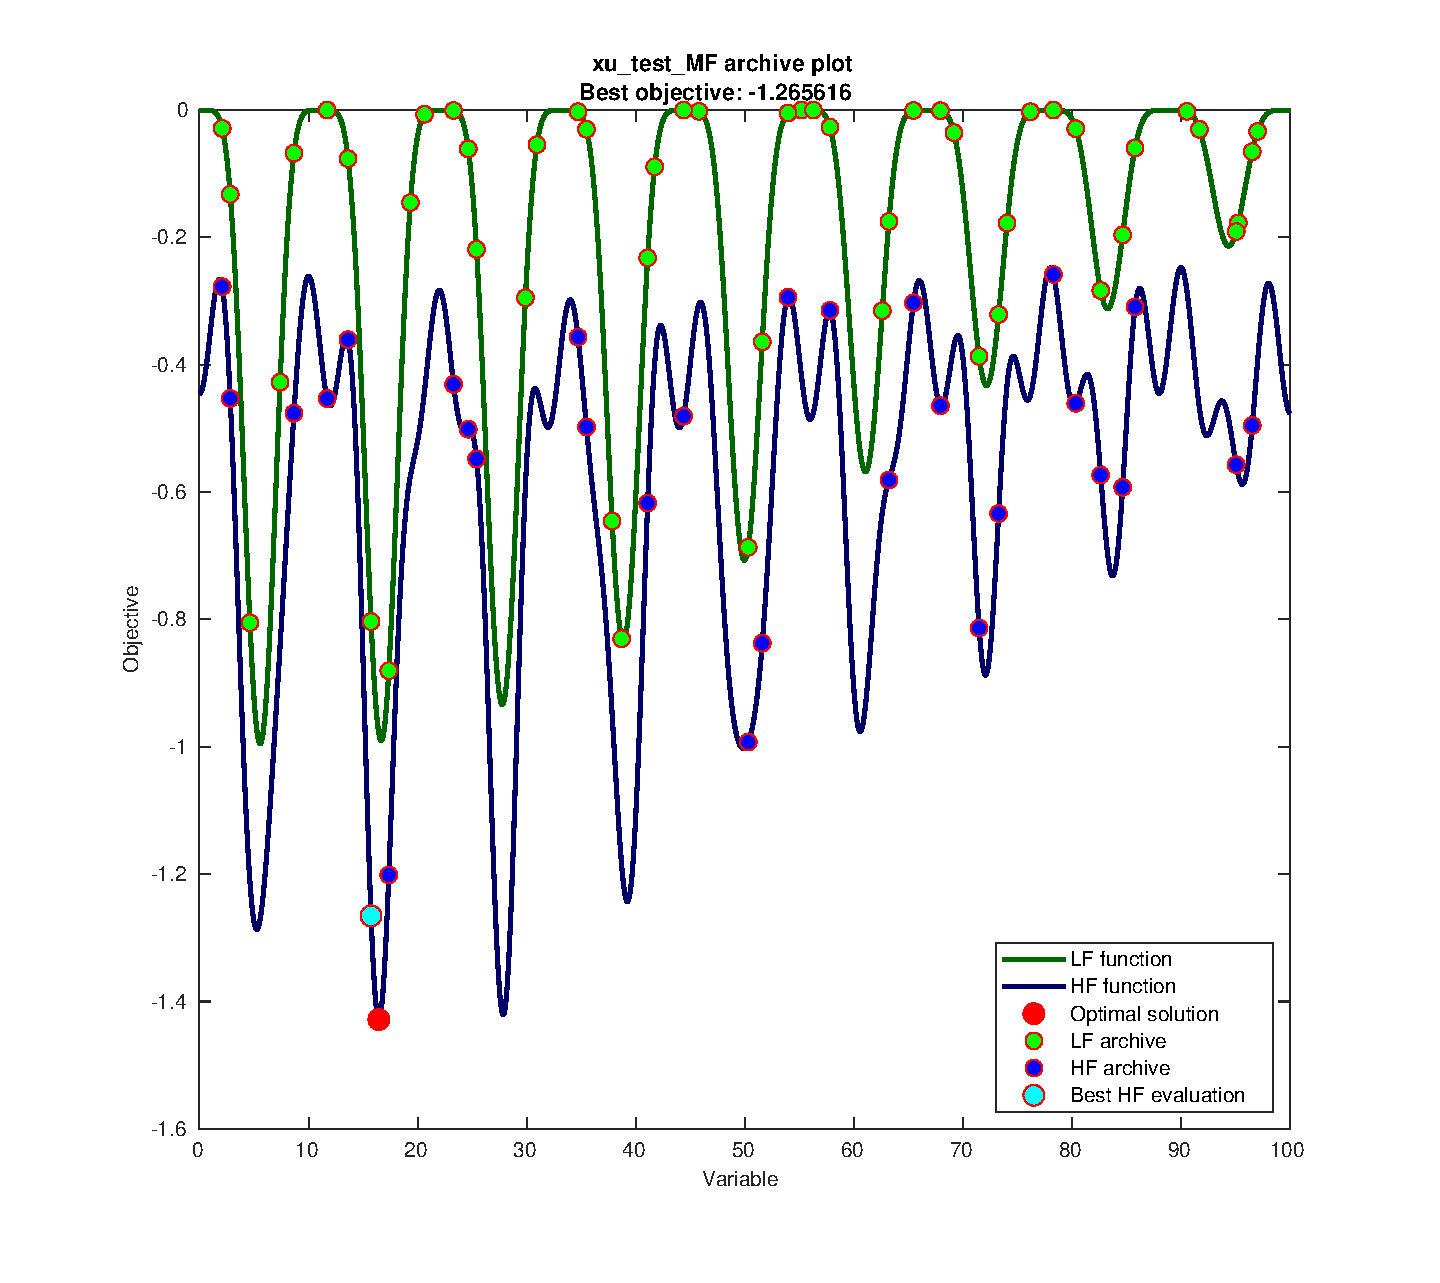
\includegraphics[width = 0.40\textwidth]{img/ex_motos.eps} 
  \caption{None of the initial low-fidelity samples is $\V{x}^*$, therefore the optimal solution cannot be obtained by \motos{}.} 
    \label{fig:motos-example}
\end{figure}
\ray{please increase axis label and legend label sizes. The top title is illegible, not too sure if you need it}In this figure, the green and the blue lines are the low- and high-fidelity response surfaces, respectively; green points are the initial low-fidelity samples; blue points are the low-fidelity samples chosen for high-fidelity evaluation; the cyan point is the best solution found; and the red point is the optimal solution, $\V{x}^*$\hemant{To the extent possible, make these points easily distinguishable. E.g. a different symbol in addition to color}\angus{will do}. It can be seen from this example that regardless of how many the initial low-fidelity samples are evaluated in high-fidelity, there is no way for \motos{} to identify the optimal solution $\V{x}^*$. The implication of this example is that \motos{} is an effective technique for choosing between a finite set of candidate solutions, but it is not as well suited to searching continuous design spaces. This shortcoming can be potentially overcome by increasing the density of the initial candidates. However, this is not trivial in terms of computational cost, and maintaining a constant density of coverage. As the number of decision variables increases exponentially, more initial samples will be required to maintain a given density; which will quickly become untenable.
